% Generated by scripts/generate_article_concordance_country_outputs.py. Do not edit.
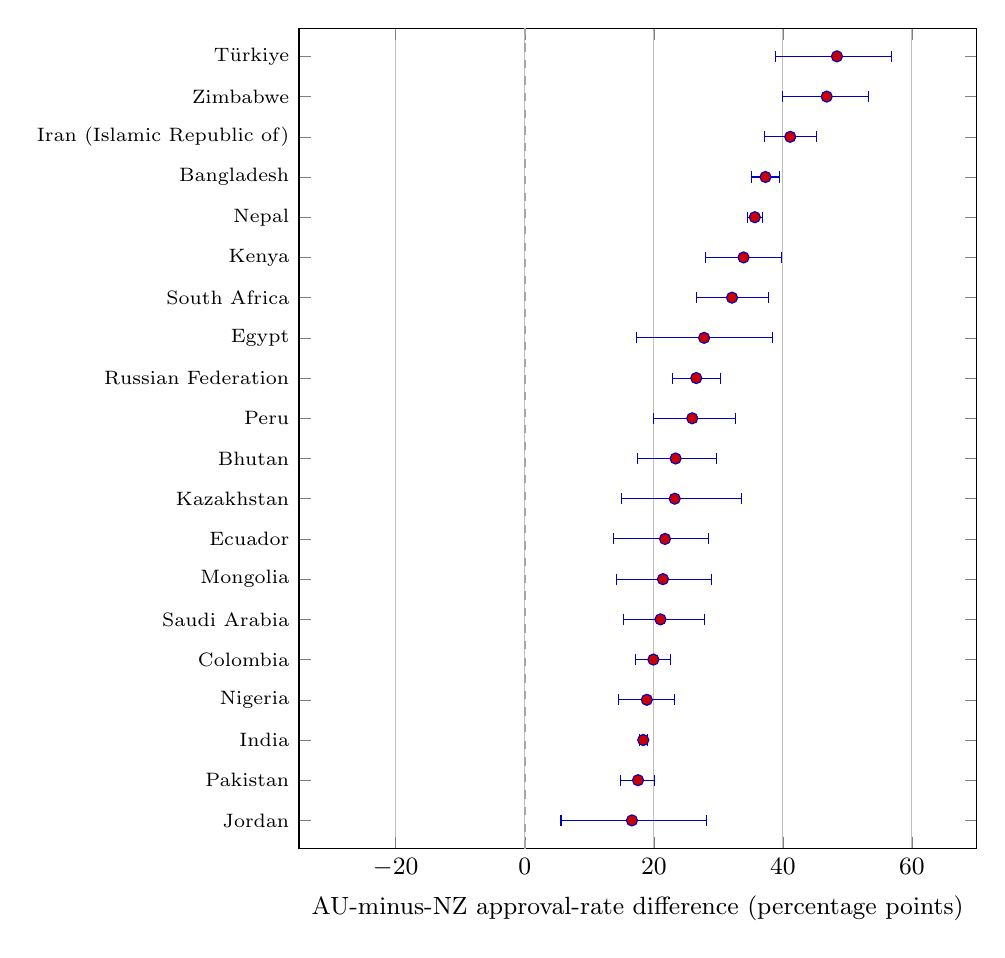
\begin{tikzpicture}
\begin{axis}[
  width=0.84\textwidth, height=12.0cm,
  xmin=-35, xmax=70, ymin=0.3, ymax=20.7,
  xlabel={AU-minus-NZ approval-rate difference (percentage points)},
  ytick={1,2,3,4,5,6,7,8,9,10,11,12,13,14,15,16,17,18,19,20}, yticklabels={{Jordan},{Pakistan},{India},{Nigeria},{Colombia},{Saudi Arabia},{Mongolia},{Ecuador},{Kazakhstan},{Bhutan},{Peru},{Russian Federation},{Egypt},{South Africa},{Kenya},{Nepal},{Bangladesh},{Iran (Islamic Republic of)},{Zimbabwe},{Türkiye}},
  y tick label style={font=\scriptsize}, tick label style={font=\small}, label style={font=\small},
  xmajorgrids=true,
]
\addplot[gray!70, dashed, thick, domain=0.3:20.7] (0,x);
\addplot+[only marks, mark=*, blue!75!black, error bars/.cd, x dir=both, x explicit] coordinates {(16.60912099,1) += (11.51301076,0) -= (10.99645407,0) (17.55112121,2) += (2.594752254,0) -= (2.653499461,0) (18.35961704,3) += (0.6022141601,0) -= (0.6009582004,0) (18.91891892,4) += (4.345113207,0) -= (4.456861073,0) (19.93365496,5) += (2.596666475,0) -= (2.755625012,0) (21.03000407,6) += (6.85650276,0) -= (5.672164601,0) (21.41615447,7) += (7.546345555,0) -= (7.147763059,0) (21.73382173,8) += (6.747087898,0) -= (8.012941349,0) (23.23979592,9) += (10.39926715,0) -= (8.316278443,0) (23.37891654,10) += (6.300089722,0) -= (5.886264785,0) (25.95820896,11) += (6.670430425,0) -= (6.038433103,0) (26.57665943,12) += (3.691616035,0) -= (3.720054153,0) (27.79363494,13) += (10.57895175,0) -= (10.51933374,0) (32.12240551,14) += (5.674233194,0) -= (5.575078282,0) (33.90681627,15) += (5.820040324,0) -= (5.920012362,0) (35.6508484,16) += (1.157550832,0) -= (1.169651141,0) (37.30485632,17) += (2.214548422,0) -= (2.194037261,0) (41.14476236,18) += (4.03601757,0) -= (4.040167521,0) (46.79504814,19) += (6.527797662,0) -= (6.917095832,0) (48.38585859,20) += (8.493884775,0) -= (9.561766232,0)};
\end{axis}
\end{tikzpicture}
